\section{Sesión 2}

\subsection{Axiomática}

\begin{enumerate}
	\item[A0:] (Axioma de vacío) Existe vacío. Notación: $\varnothing$.
	\item[A1:] (Axioma de extensión) $\forall x (x\in A \iff x\in B)\implies A =B$. 
	\item[A2:] (Esquema axiomático de separación) $\exists B\ \forall x \ni (x\in B\iff [x\in A\wedge \Phi(x)])$.
\end{enumerate}

\begin{definicion}(Conjunto)
	$y$ es conjunto $\iff(\exists x(x\in y))\vee (y=\varnothing)$. 
\end{definicion}

\begin{definicion}(No pertenencia)
	$x\not\in y \iff \neg (x\in y)$. 
\end{definicion}

\begin{teorema}
	$\forall x,x\not\in \varnothing$. 
\end{teorema}

\begin{teorema}
	$\forall x, x\not\in A \iff A=\varnothing$. 
\end{teorema}

\begin{definicion}(Contención)
	$A\subseteq B\iff \forall x(x\in A\implies x\in B)$. 
\end{definicion}

\begin{definicion}(Contención estricta)
	$A \subset B\iff(A\subseteq B\wedge A\neq B)$.
\end{definicion}

\begin{teorema}
	$A\subseteq \varnothing\implies A = \varnothing$. 
\end{teorema}

\begin{teorema}
	$\neg (A\subset A)$. 
\end{teorema}


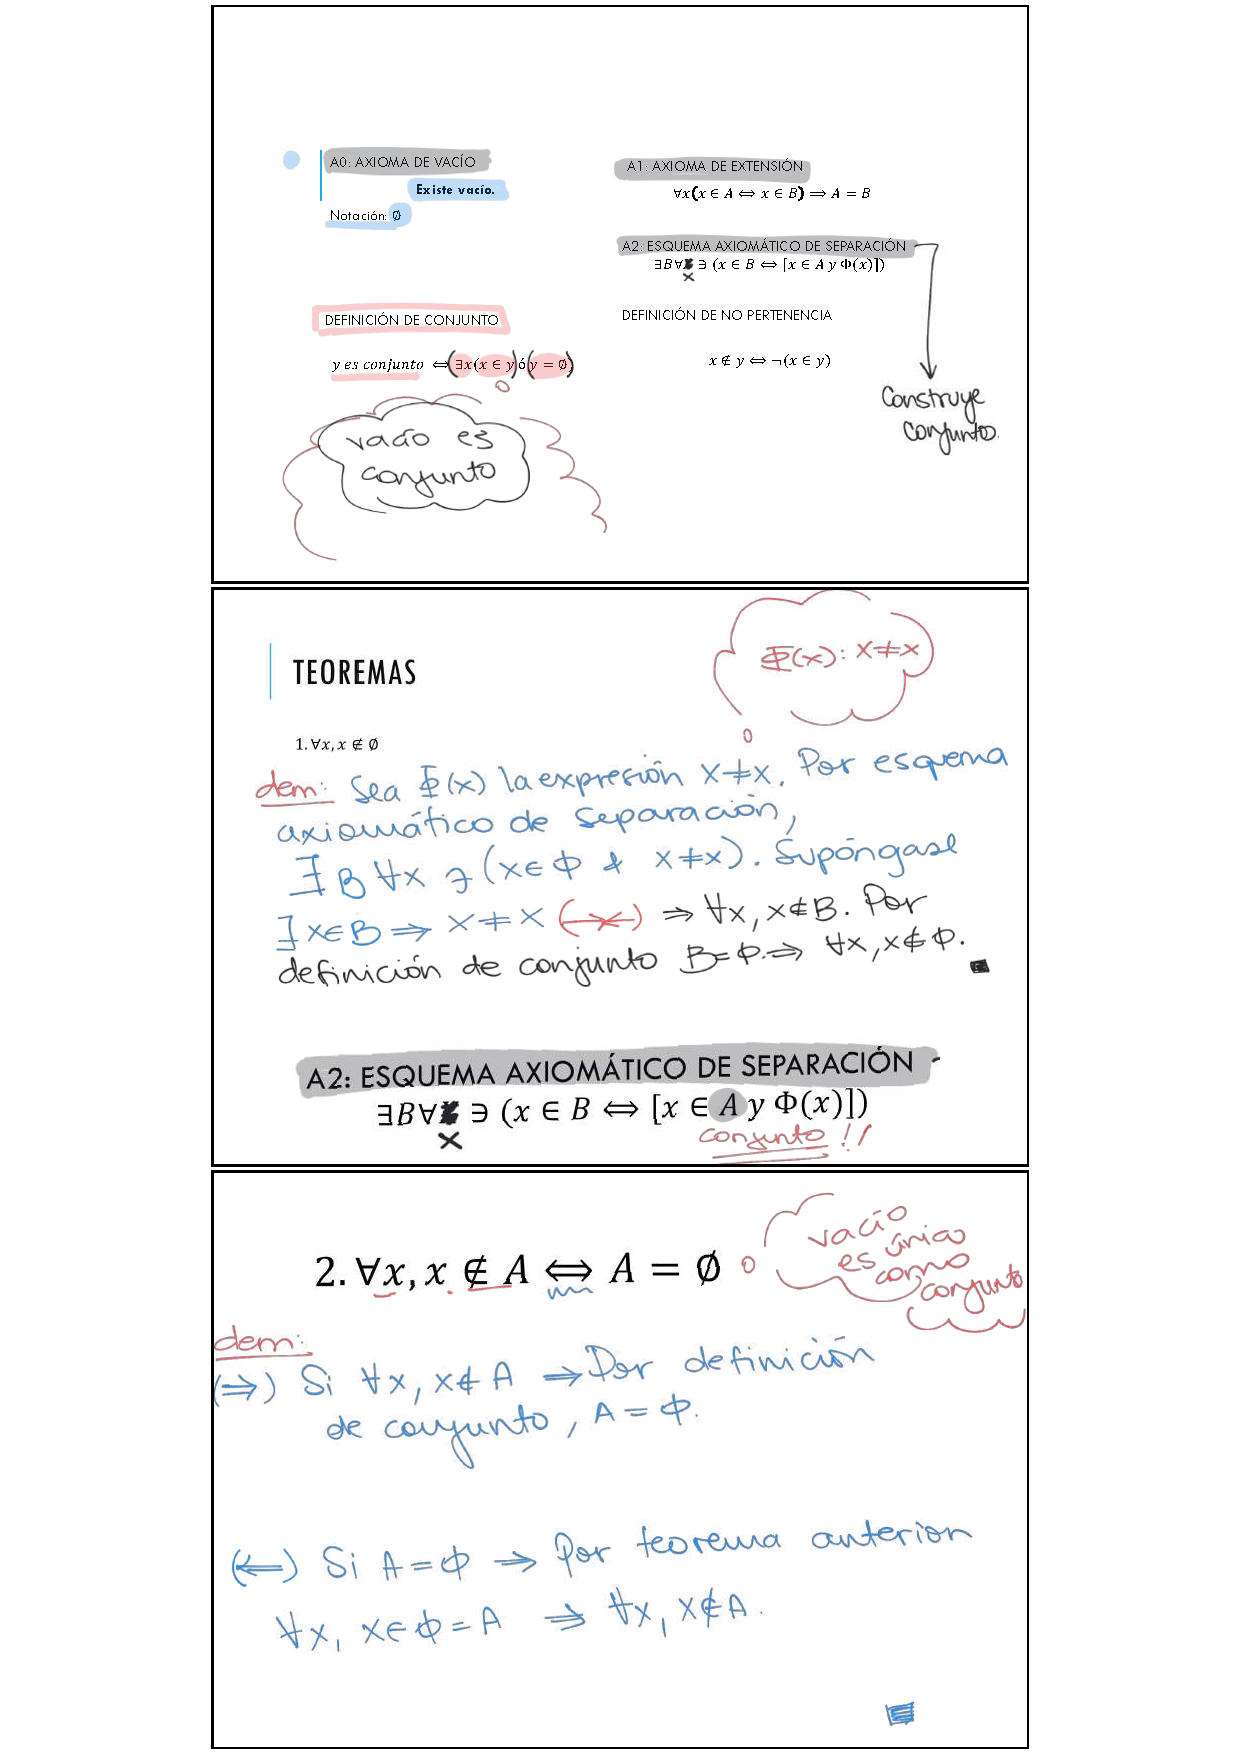
\includepdf[pages=-]{Apendices/s2.pdf}